




%---------------------------------------------------------------------

\newpage

%\section[Co-evolution at the meso scale][Co-évolution à l'échelle mesoscopique]{Co-evolution of forms: interactions and morphogenesis at the meso scale}{Co-evolution des formes : interactions et morphogenèse à l'échelle mesoscopique}

\section{Co-evolution at the meso scale}{Co-évolution à l'échelle mesoscopique}


\label{sec:mesocoevolmodel}

%---------------------------------------------------------------------


\bpar{
Urban settlements and transportation networks are widely admitted to be co-evolving in the thematic and empirical studies of territorial systems. However, modeling approaches of such dynamical interactions between networks and territories are less developed. We propose to study this issue at an intermediate scale, focusing on morphological and functional properties of the territorial system in a stylized way. We introduce a stochastic dynamical model of urban morphogenesis that couples the evolution of population density within grid cells with a growing road network.
}{
Les établissements urbains et les réseaux de transport ont été montrés comme co-évolutif, dans les différentes approches thématiques, empiriques, et de modélisation des systèmes territoriaux développées jusqu'ici. Comme on l'a vu, les approches modélisant ces interactions dynamiques entre réseaux et territoires sont peu développées. Nous proposons dans cette section de réaliser une première entrée à une échelle intermédiaire, en s'intéressant aux propriétés morphologiques et fonctionnelles des systèmes territoriaux de manière stylisée. Nous introduisons un modèle dynamique et stochastique de morphogenèse urbaine qui couple l'évolution de la densité de population dans les cellules d'une grille avec un réseau routier croissant.
}


%%%%%%%%%%%%%%%%%%
\subsection{Model}{Modèle}




\paragraph{Rationale}{Rationelle}



\bpar{
With an overall fixed growth rate, new population aggregate preferentially to a potential for which parameters control the dependance to various explicative variables, namely local density, distance to the network, centrality measures within the network and generalized accessibility. We generalize thus the morphogenesis model studied in~\ref{sec:densitygeneration} with aggregation mechanisms similar to~\cite{raimbault2014hybrid}.
A continuous diffusion of population completes the aggregation to translate repulsion processes generally due to congestion. Because of the different time scales of evolution for urban scape and networks, the network grows at fixed time steps, with rules that can be switched in a multi-modeling fashion. A fixed rule ensure connectivity of newly populated patches to the existing network.
%Two different heuristics are then compared: one based on gravity potential breakdown for which links are created if a generalized interaction potential through a new candidate link exceeds a certain times the potential within the existing network; a second one implementing biological network growth, more precisely a slime mould model.
The different network generation heuristics introduced in~\ref{sec:networkgrowth} are included in the model.
We expect the different heuristics to be complementary since the gravity model would be more typical of planned top-down network evolution, whereas the biological model will translate bottom-up processes of network growth. 
}{
Les principes généraux du modèle sont les suivants. Avec un taux de croissance global fixé, une nouvelle population s'agrège préférentiellement à un potentiel local, dont la dépendance à diverses variables explicatives est contrôlé par des paramètres. Celles-ci sont la densité locale, la distance au réseau, les mesures de centralité dans le réseau et l'accessibilité généralisée. \cite{doi:10.1080/13658816.2014.893347} montre dans le cas de Stockholm la très forte corrélation entre les différents types de centralité et le type d'usage du sol, ce qui confirme l'importance de considérer les centralités comme variables explicatives pour le modèle à cette échelle. Nous généralisons ainsi le modèle de morphogenèse étudié dans~\ref{sec:densitygeneration}, avec des mécanismes d'agrégation similaires à ceux utilisés par~\cite{raimbault2014hybrid}. Une diffusion continue de la population complète l'agrégation pour traduire les processus de répulsion généralement dus à la congestion. A cause des différentes échelles de temps impliquées dans l'évolution de l'environnement urbain et des réseaux, le réseau croit à pas de temps fixes, suivant le sous-modèle développé en~\ref{sec:networkgrowth} : une première règle fixe assure la connectivité des patches nouvellement peuplés au réseau existant. Les différentes heuristiques de génération de réseau sont ensuite incluses dans le modèle. Nous nous attendons à une complémentarité de celles-ci, puisque par exemple le modèle gravitaire sera plus typique d'une évolution de réseau planifiée, tandis que le modèle biologique traduit des processus auto-organisés de croissance de réseau. La Fig.~\ref{fig:mesocoevolmodel:workflow} résume la structure générale du modèle de morphogenèse.
}




%%%%%%%%%%%%%%%
\begin{figure}
	\includegraphics[width=\linewidth]{Figures/MesoCoEvol/mesocoevol}
	\caption[][Morphogenèse mesoscopique]{}{\textbf{Workflow du modèle de co-évolution à l'échelle mesoscopique.}\label{fig:mesocoevolmodel:workflow}}
\end{figure}
%%%%%%%%%%%%%%%



\paragraph{Formalization}{Formalisation}

Patch utility given by $U_i = \sum_k w_k \cdot \tilde{x}_k$ with $\tilde{x}_k$ normalized local variables among population, betweenness and closeness centrality, distance to roads, accessibility ; aggregation done with probability $\left(U_i/\sum_k U_k\right)^\alpha$ ; diffusion among neighbors $n_d$ times with strength $\beta$.


%%%%%%%%%%%%%%%%%%%
\subsection{Results}{Résultats}


\subsubsection{Static and Dynamical calibration}{Calibration statique et dynamique}



\bpar{
The model is calibrated at the first order (indicators of urban form and network measures) and at the second order (correlations) with Eurostat population grid coupled with street network from OpenStreetMap through the following workflow: indicators (Moran index, mean distance, hierarchy, entropy for morphology, mean path length, centralities, performance for network) are computed on real areas of width 50km for all Europe (what corresponds to the typical scale of processes the model includes); parameter space of the model is explored using grid computing (with OpenMole model exploration software), from simple synthetic initial configurations (few connected punctual settlements), computing indicators on final simulated configurations; among candidate parameters for given contiguous (in space and indicator space) real areas on which correlations can be computed, the one with the closest correlation matrix computed on repetitions is chosen.
}{
Le modèle est calibré au premier ordre, sur les indicateurs de forme urbaine et de mesure de réseau, ainsi qu'au second ordre sur les correlations entre ceux-ci. Les données réelles utilisées sont toujours celles introduites en~\ref{sec:staticcorrelations}, basées sur les données de population raster Eurostat et le réseau routier issu d'OpenStreetMap. Le processus de calibration est le suivant :
}



La Fig.~\ref{fig:mesocoevolmodel:calibration} résume les résultats de la calibration.


We obtain a full coverage of real configurations with simulation results in a principal component plan for indicators, for which most of them a close correlation structure is found. Both network heuristics are necessary for the full coverage. The model is thus able to reproduce existing urban form and networks, but also their \emph{interaction} in the sense of correlations.




%%%%%%%%%%%%%%%
\begin{figure}
	%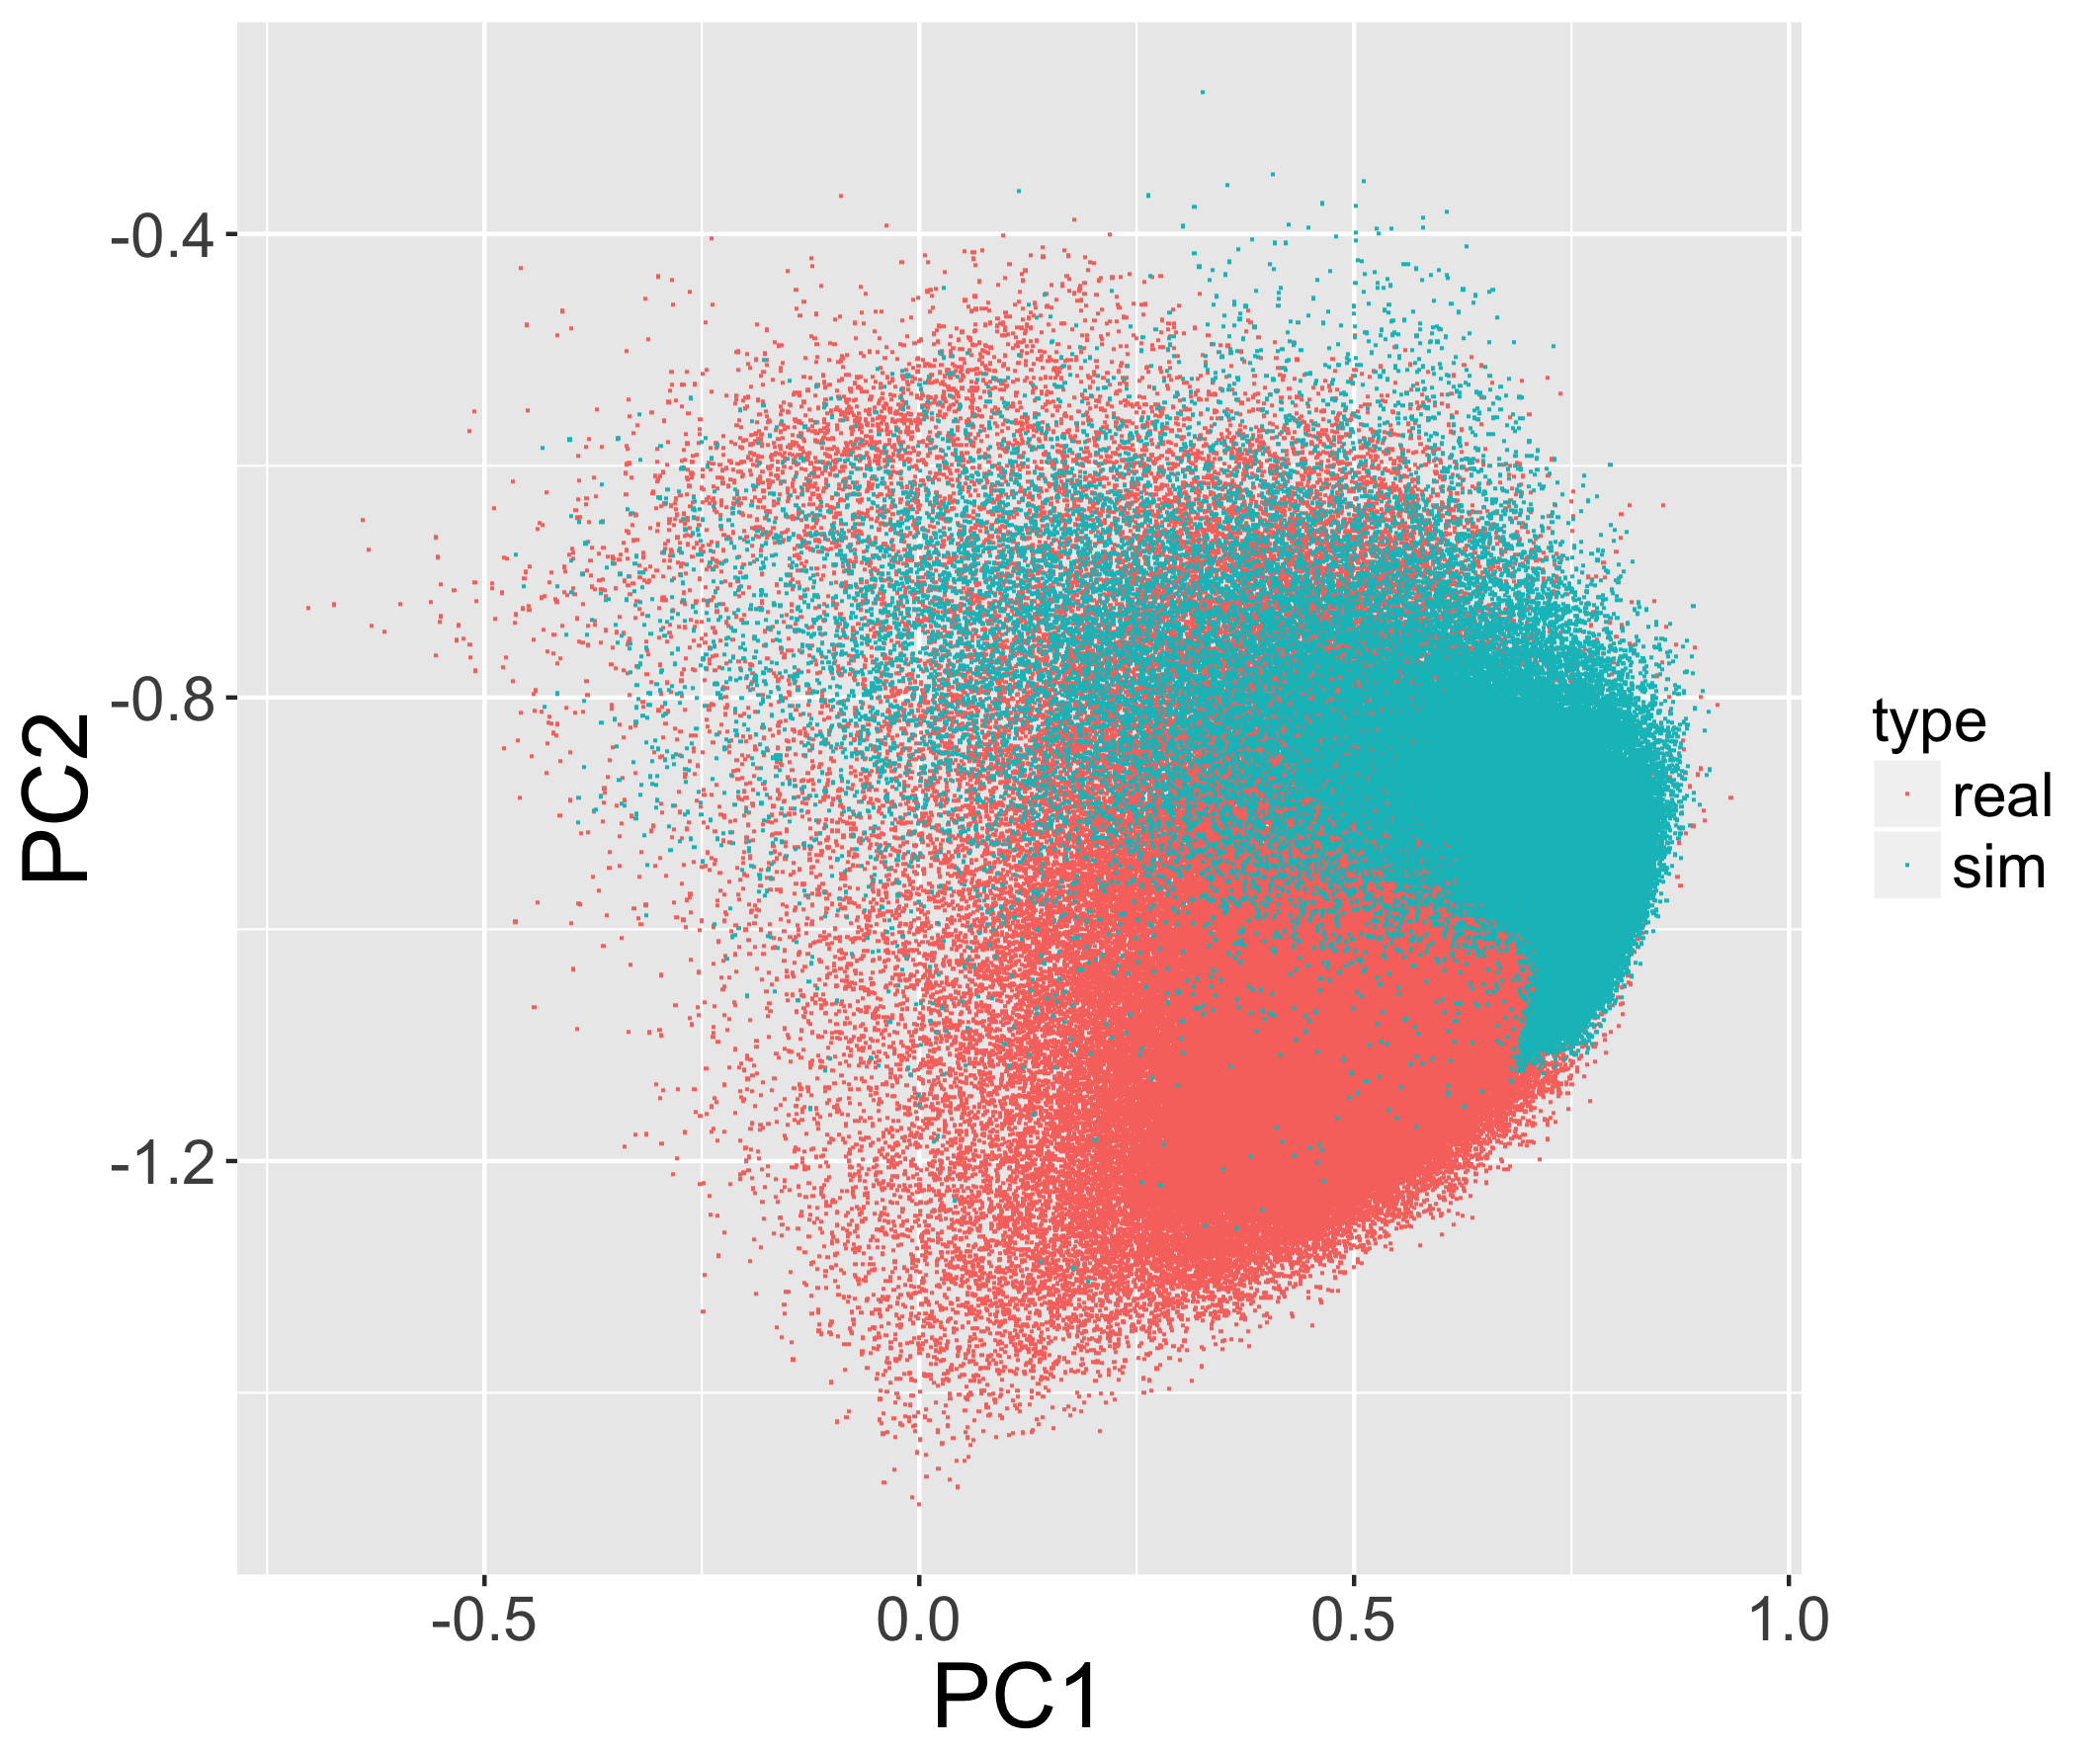
\includegraphics[width=0.48\linewidth]{Figures/MesoCoEvol/pca_allobjs}
	%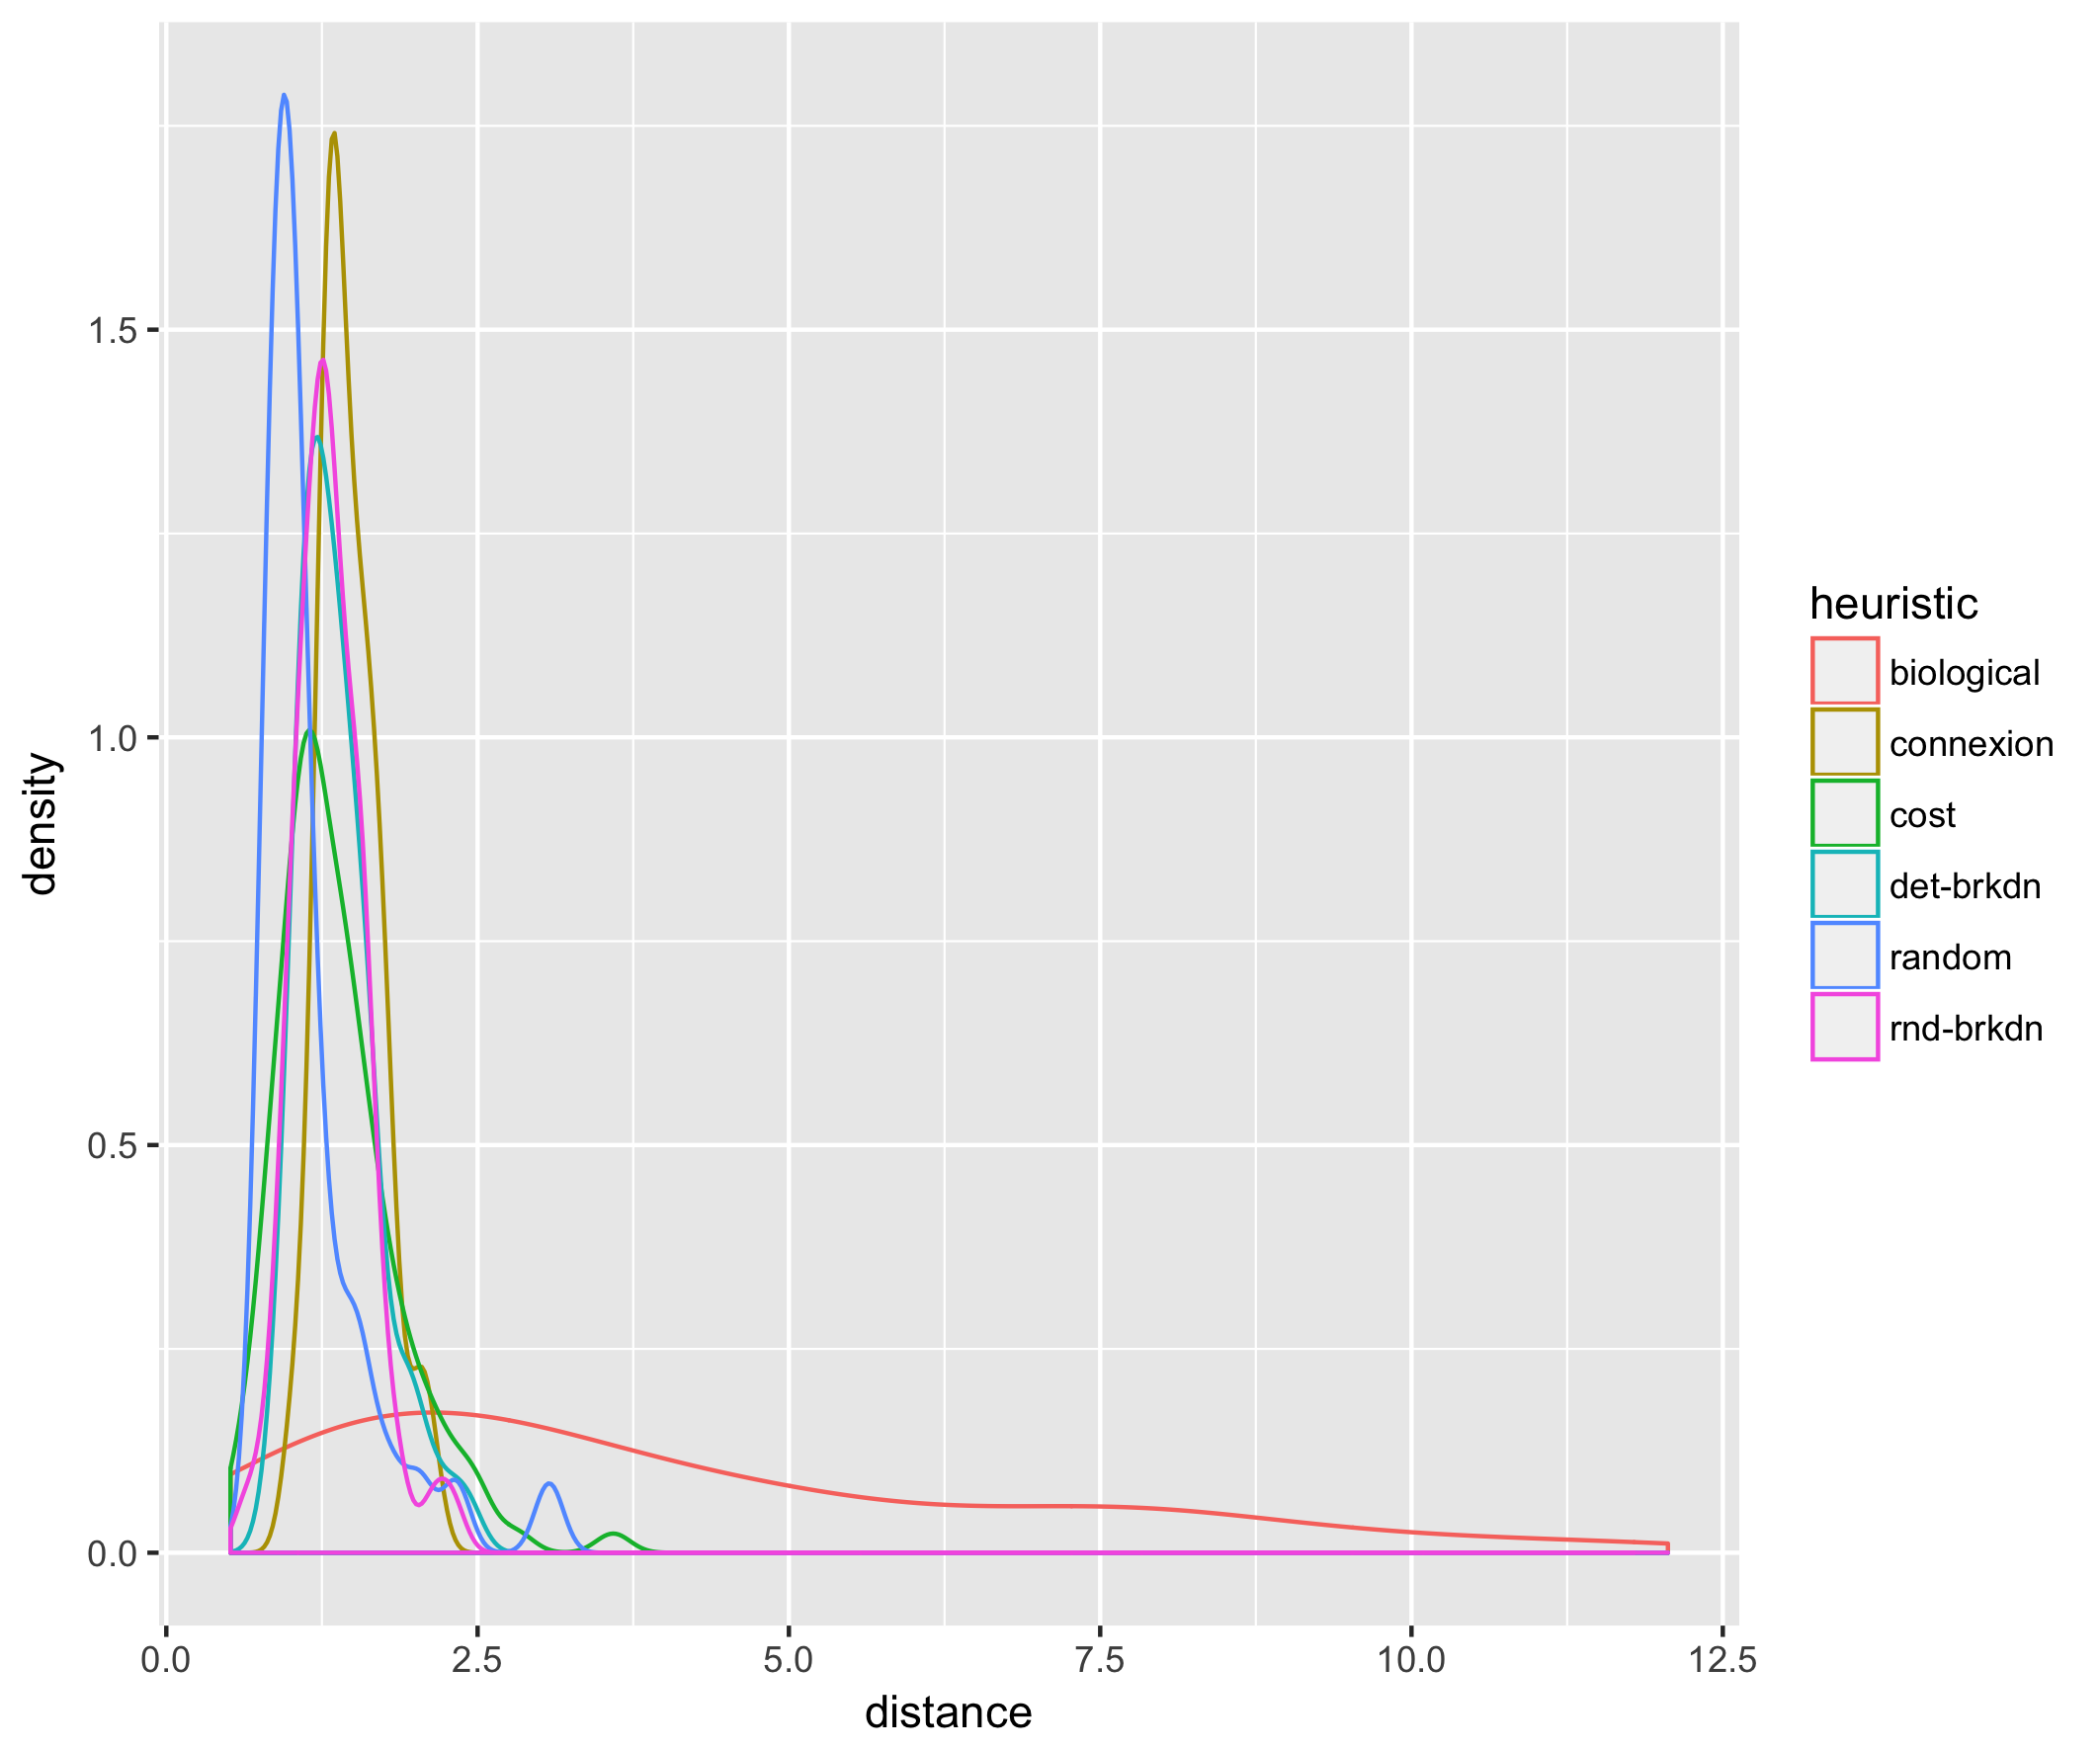
\includegraphics[width=0.48\linewidth]{Figures/MesoCoEvol/corrs-distrib_rhoasize4.png}\\
	%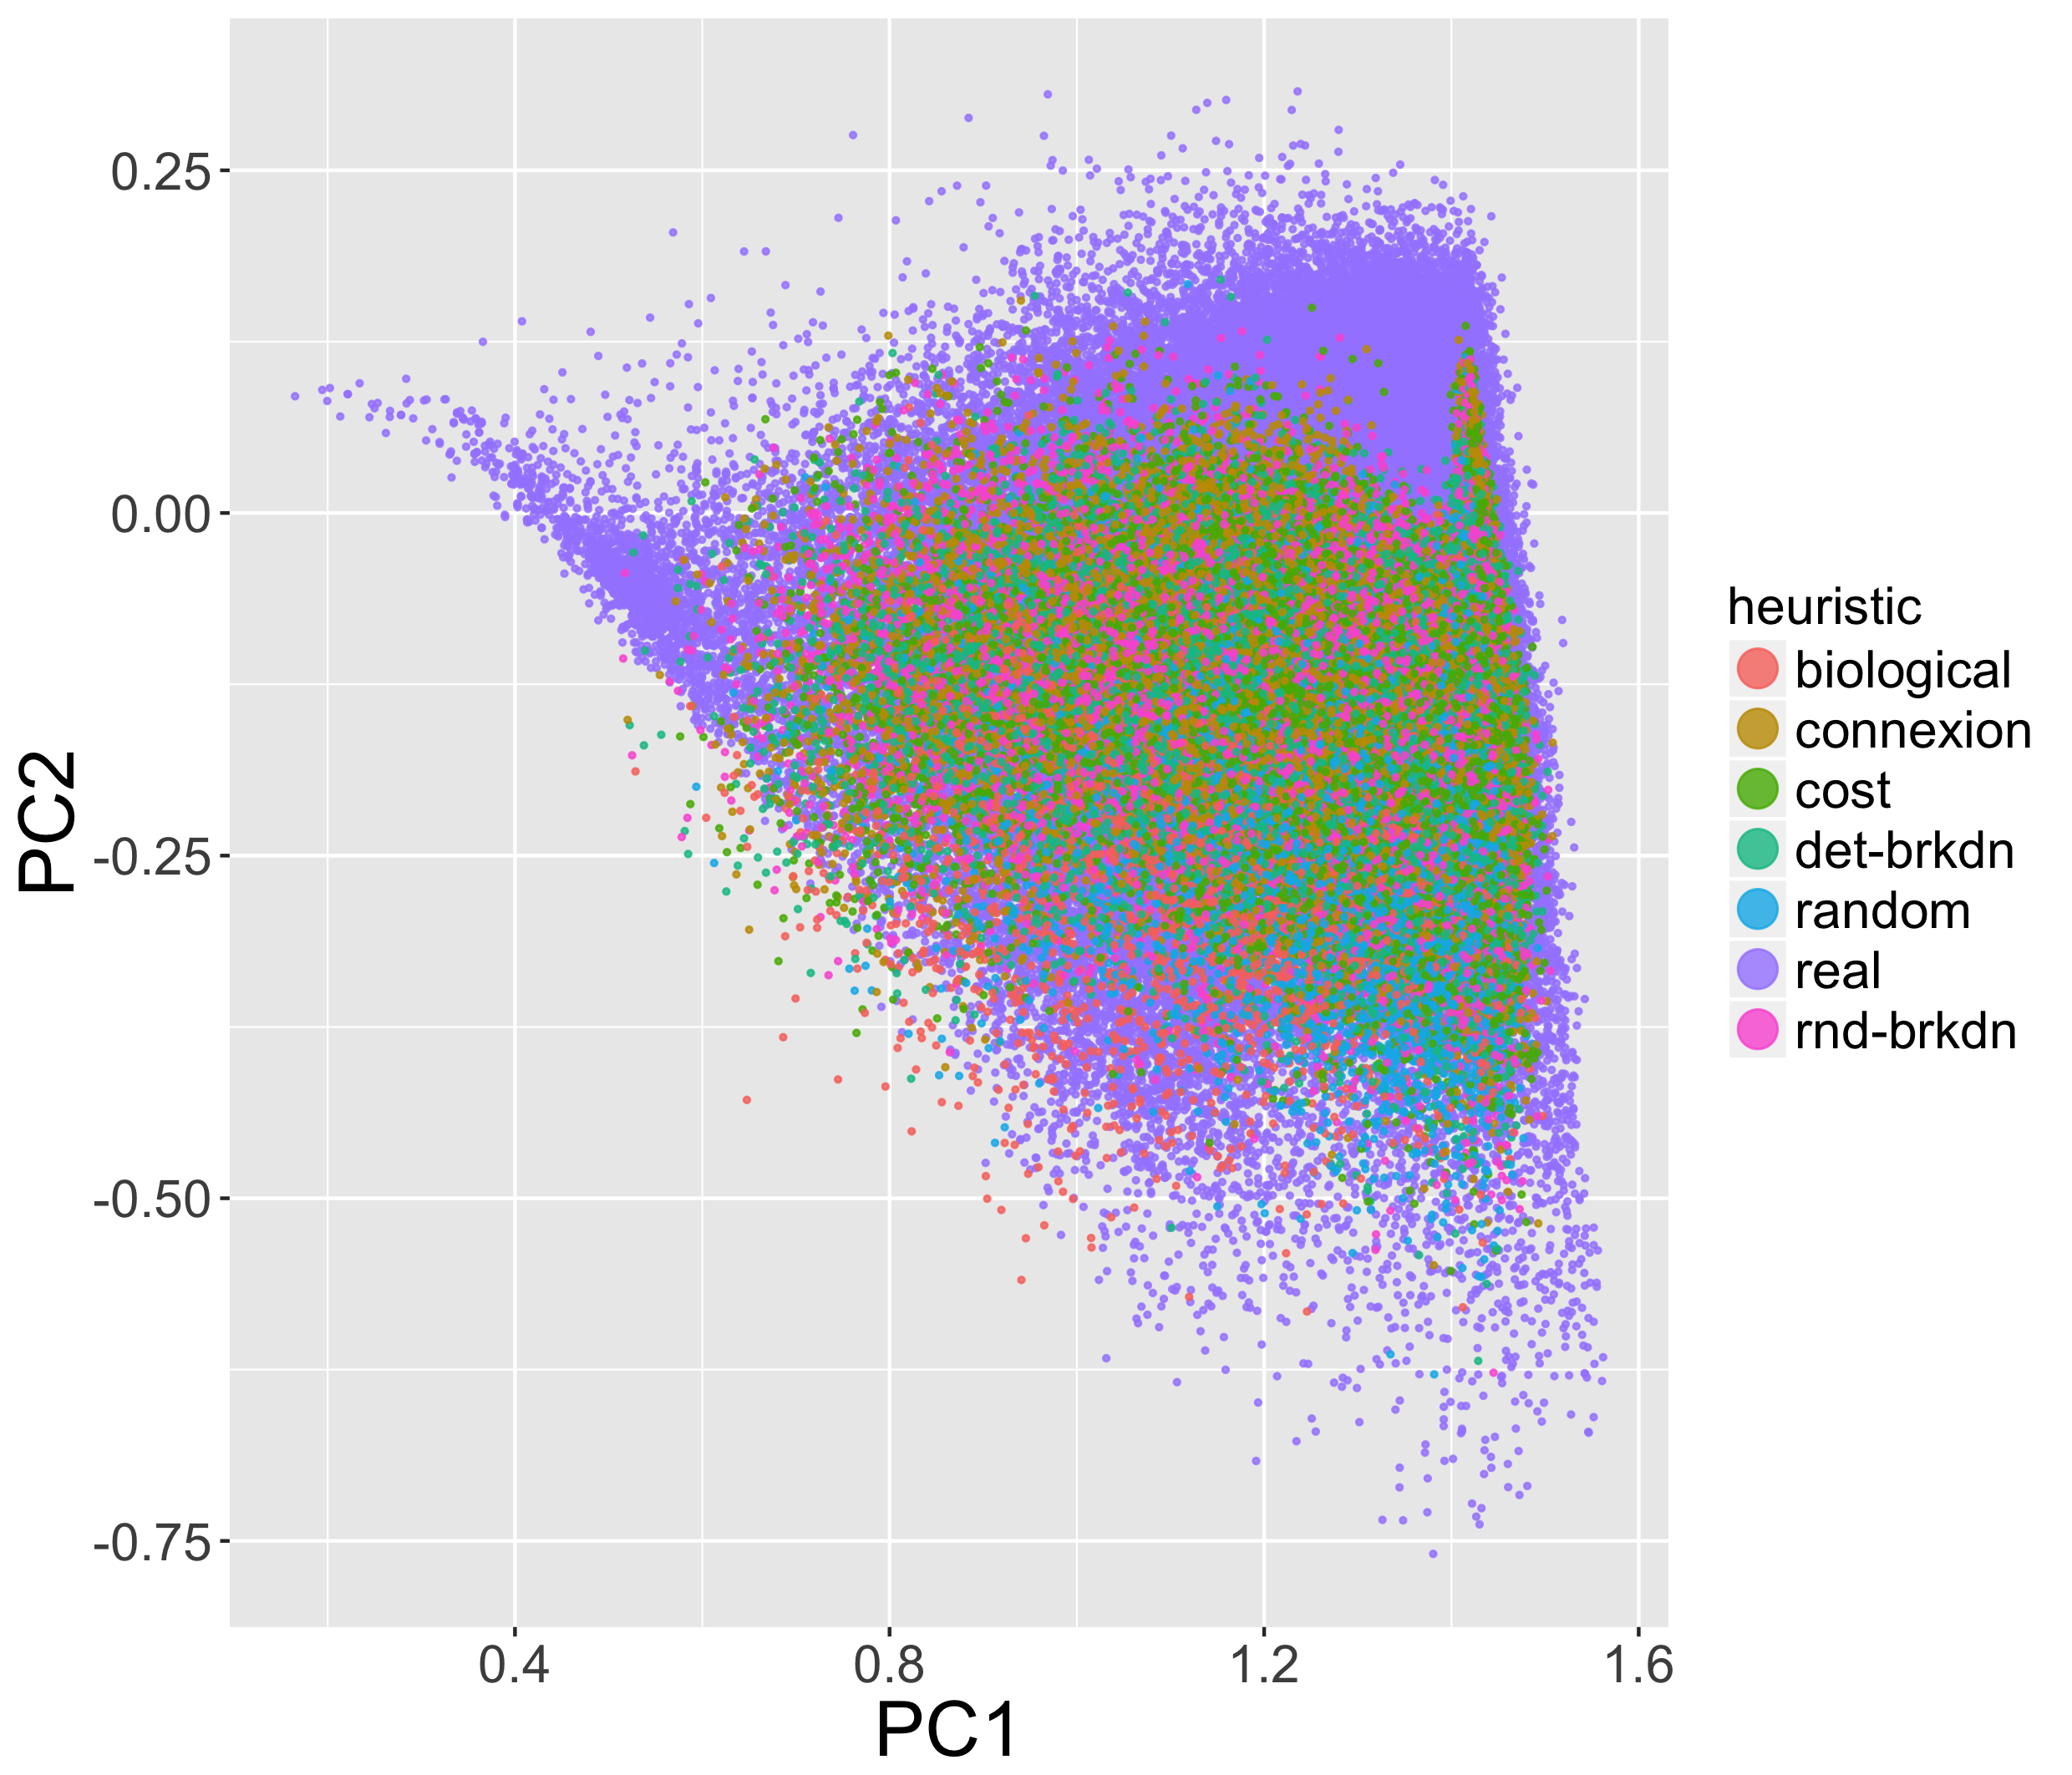
\includegraphics[width=0.48\linewidth]{Figures/MesoCoEvol/pca_morpho_byheuristic}
	%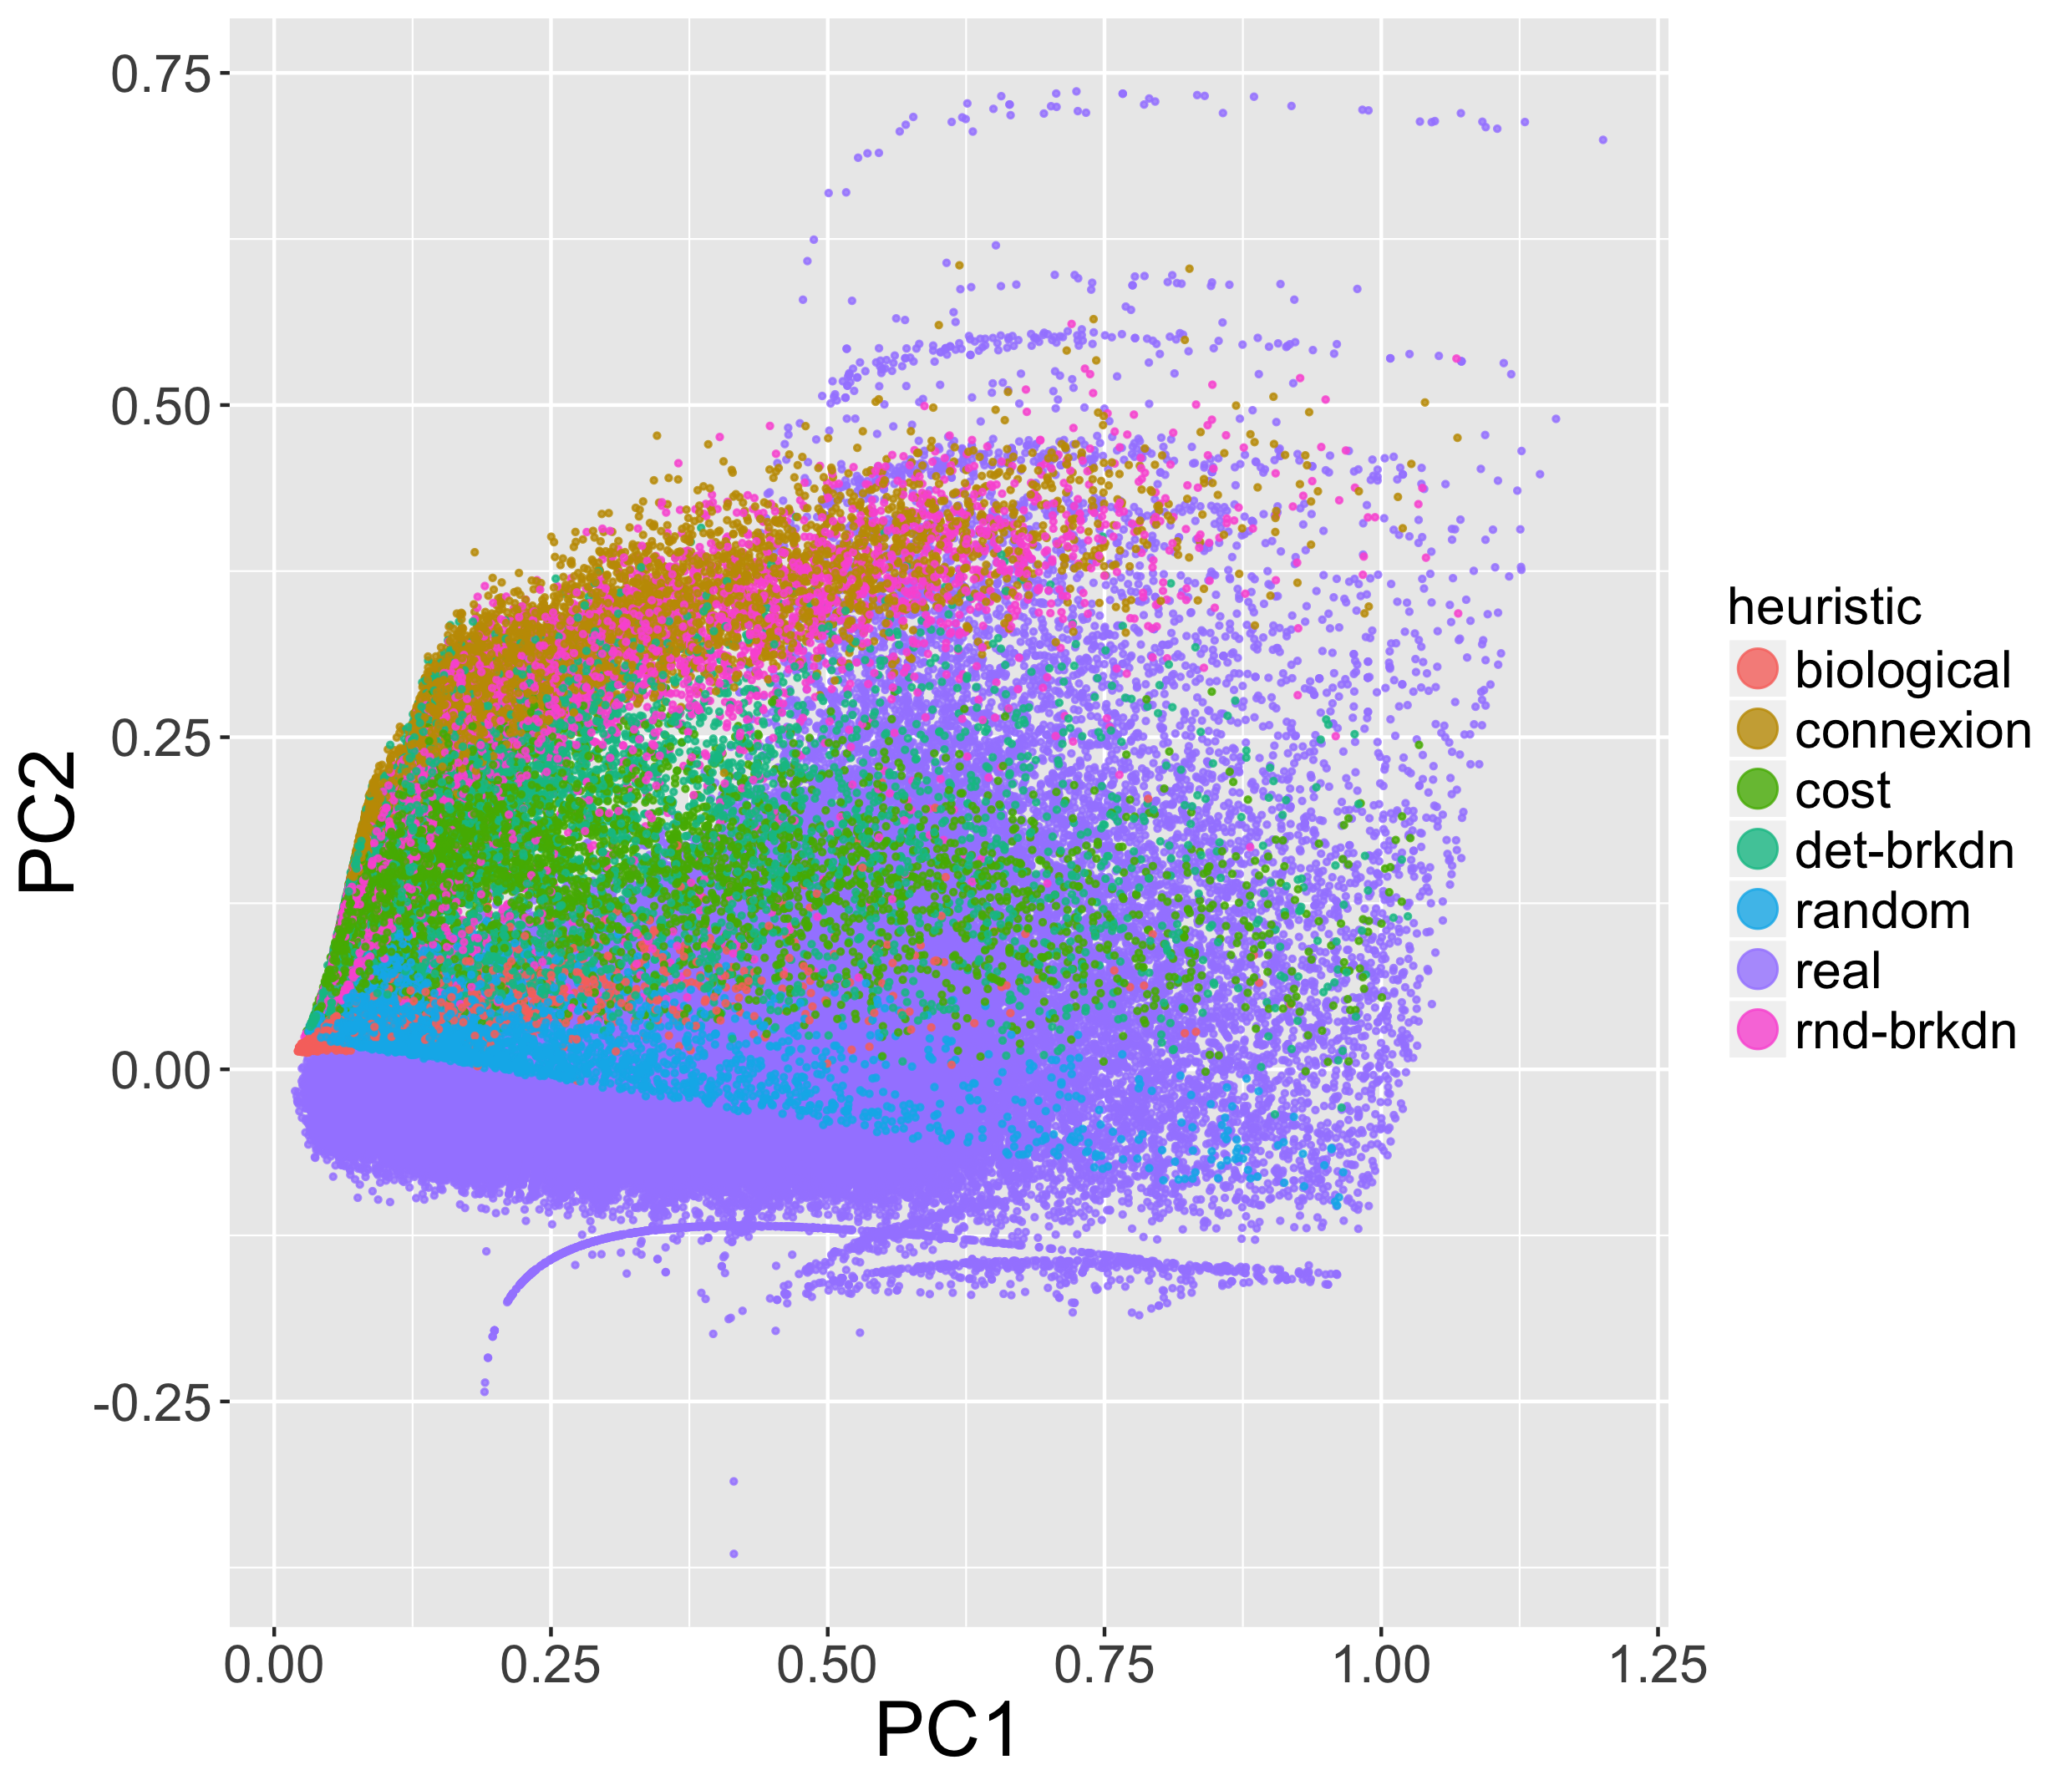
\includegraphics[width=0.48\linewidth]{Figures/MesoCoEvol/pca_network_byheuristic}
	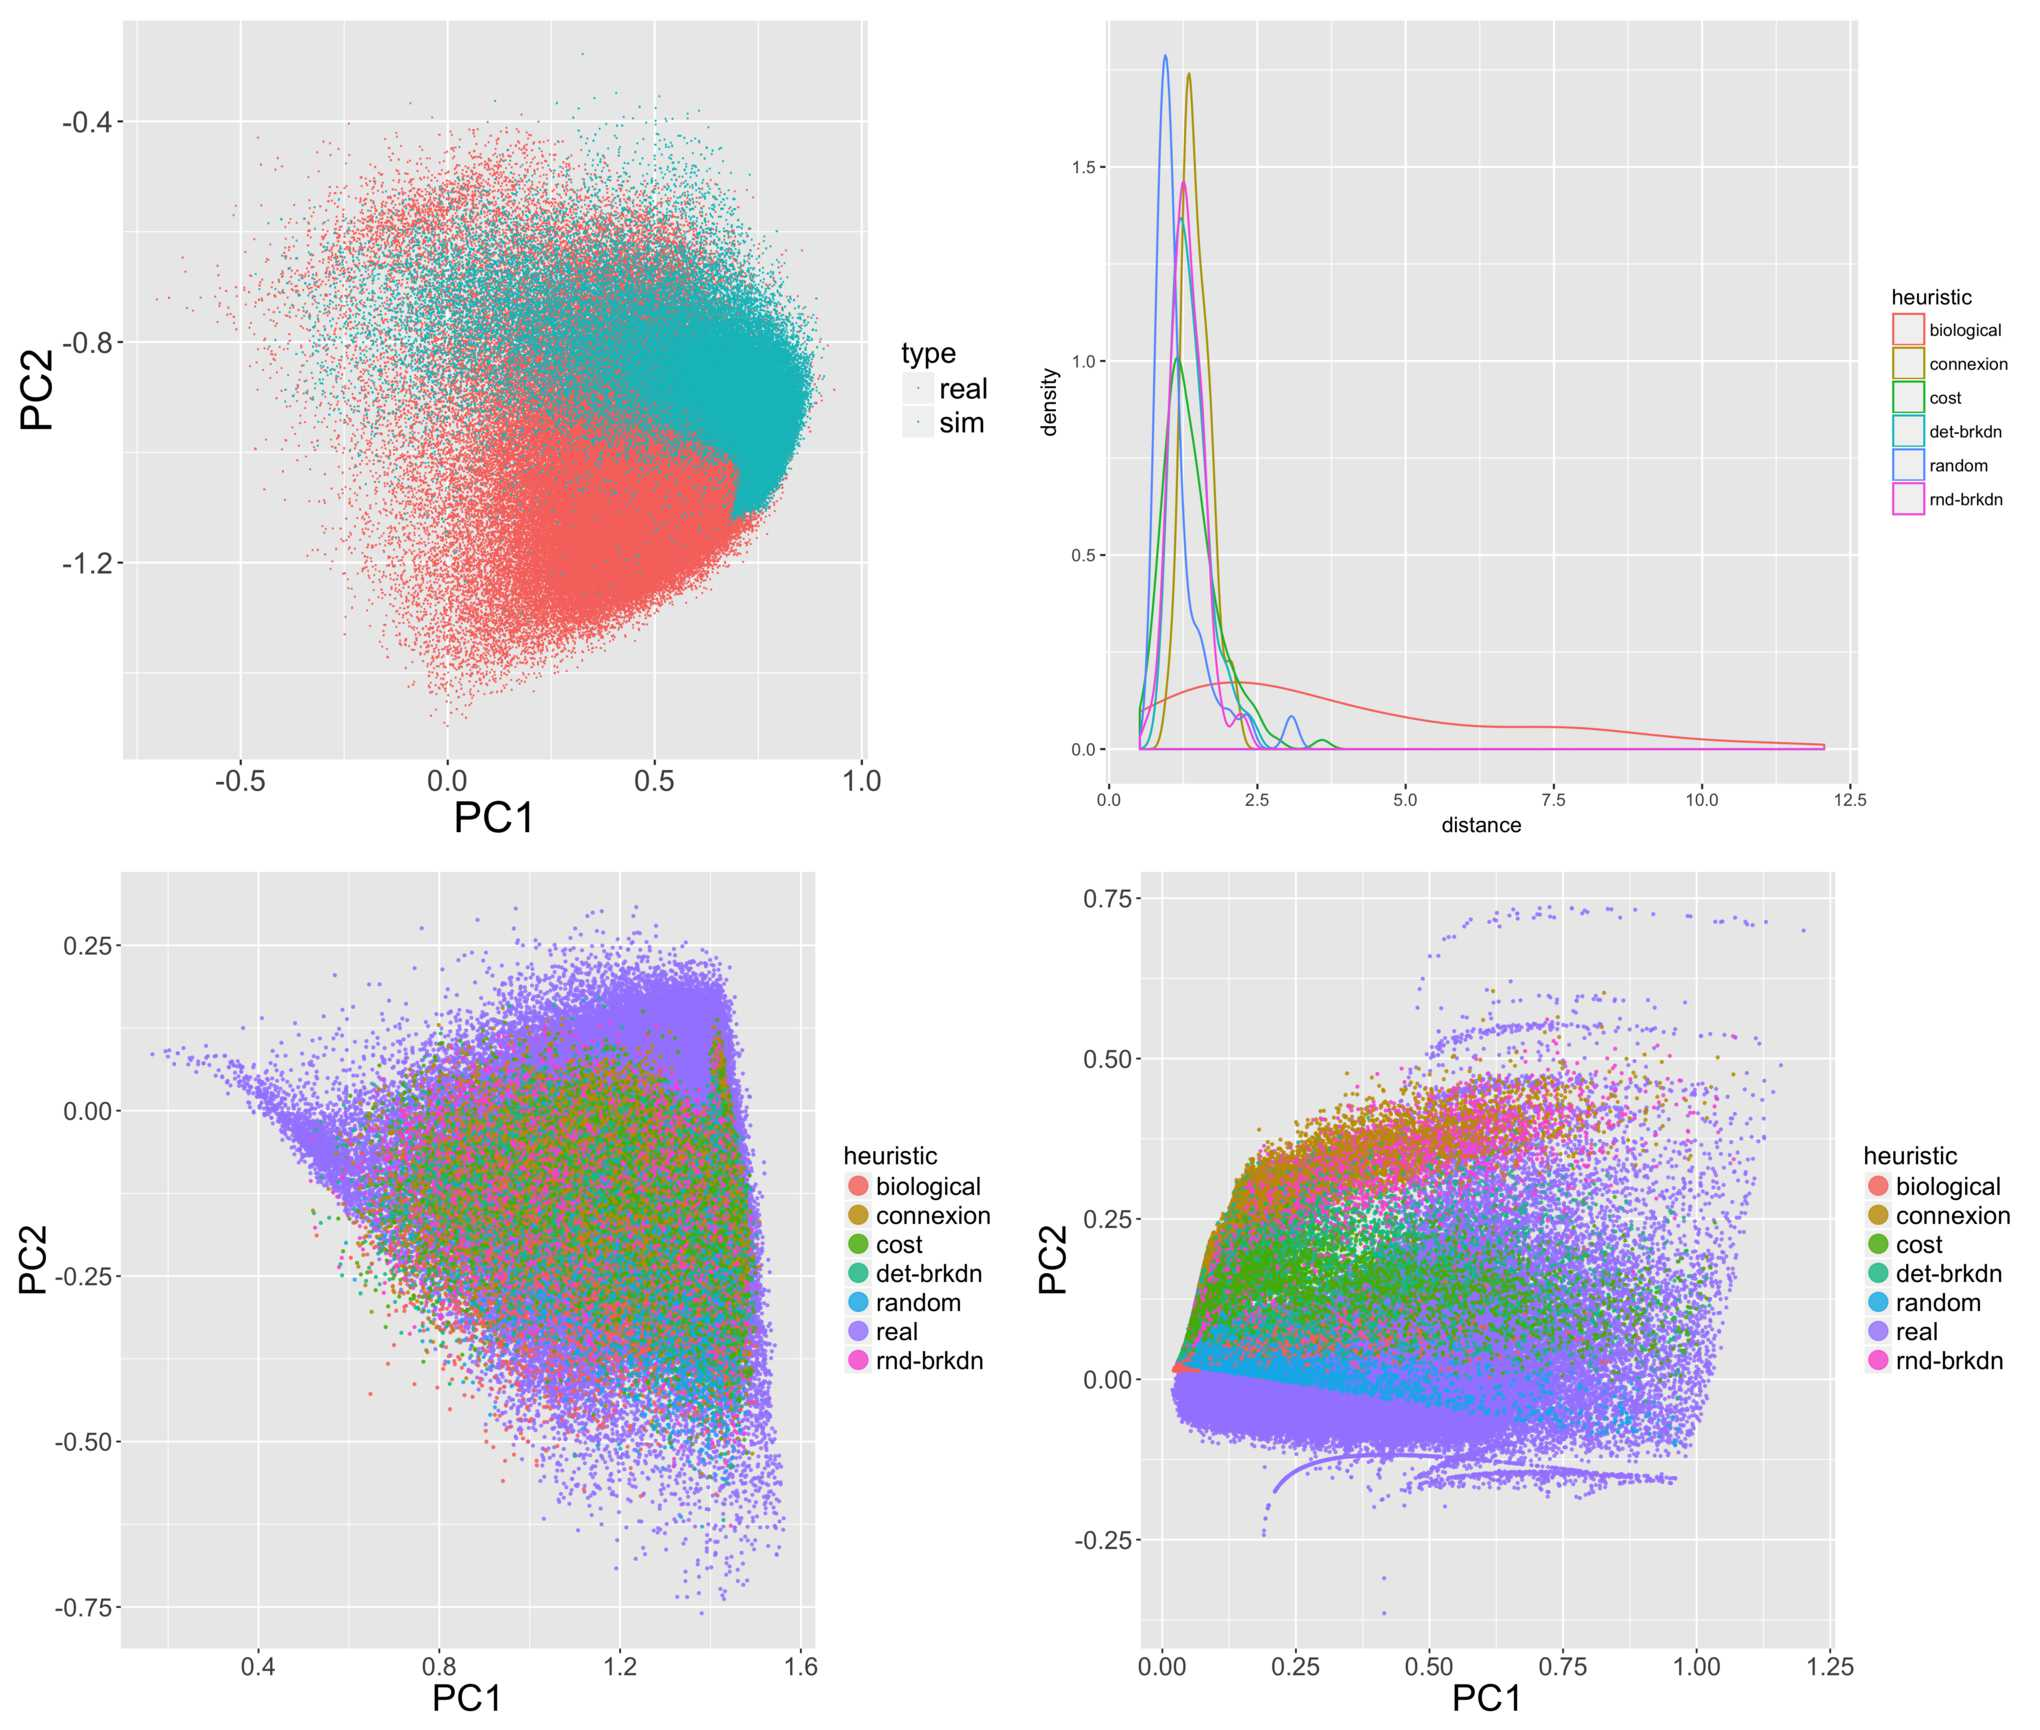
\includegraphics[width=\textwidth]{Figures/Final/7-2-2-fig-mesocoevolmodel-calibration.jpg}
	\caption[Morphogenesis model calibration][Calibration du modèle de morphogenèse]{\label{fig:mesocoevolmodel:calibration}}{\textbf{Calibration du modèle de morphogenèse au premier et au second ordre.}\label{fig:mesocoevolmodel:calibration}}
\end{figure}
%%%%%%%%%%%%%%%





\subsubsection{Causality Regimes}{Régimes de causalité}



\bpar{
We furthermore study dynamical lagged correlations between normalized returns of population and network patch explicatives variables, exhibiting a large diversity of spatio-temporal causality regimes, where network can drive urban growth, the contrary, or more complex circular causalities, suggesting that the model effectively grasps the dynamical richness of interactions.
}{
Nous étudions d'autre part les correlations retardées dynamiques entre les retours normalisés de la population et des variables explicatives des patches, appliquant la méthode des régimes de causalité introduite en~\ref{sec:causalityregimes}. Le modèle exhibe des régimes de causalité divers. Plus précisément, la Fig.~\ref{fig:mesocoevolmodel:causality} résume les résultats obtenus. Le nombre de classe induisant une transition est plus faible que pour le modèle RDB, traduisant un plus faible degré de liberté, et nous fixons dans ce cas $k=4$. Les profils des centroïdes permettent de comprendre
}

% incluant des causalité circulaires, suggérant qu'il capture effectivement la richesse des interactions dynamiques
% reg 1 : network suit pop ; reg 2 : idem mais pas dans strucutre locale (pop road $\simeq 0$) ; reg3 : nw suit mais que local, pas structure. ; reg 4 : bw anticause access : network and pop avoid congestion ; plus nw suit : somehow circulaire, vraie co-evol ?


%%%%%%%%%%%%%%%
\begin{figure}
	%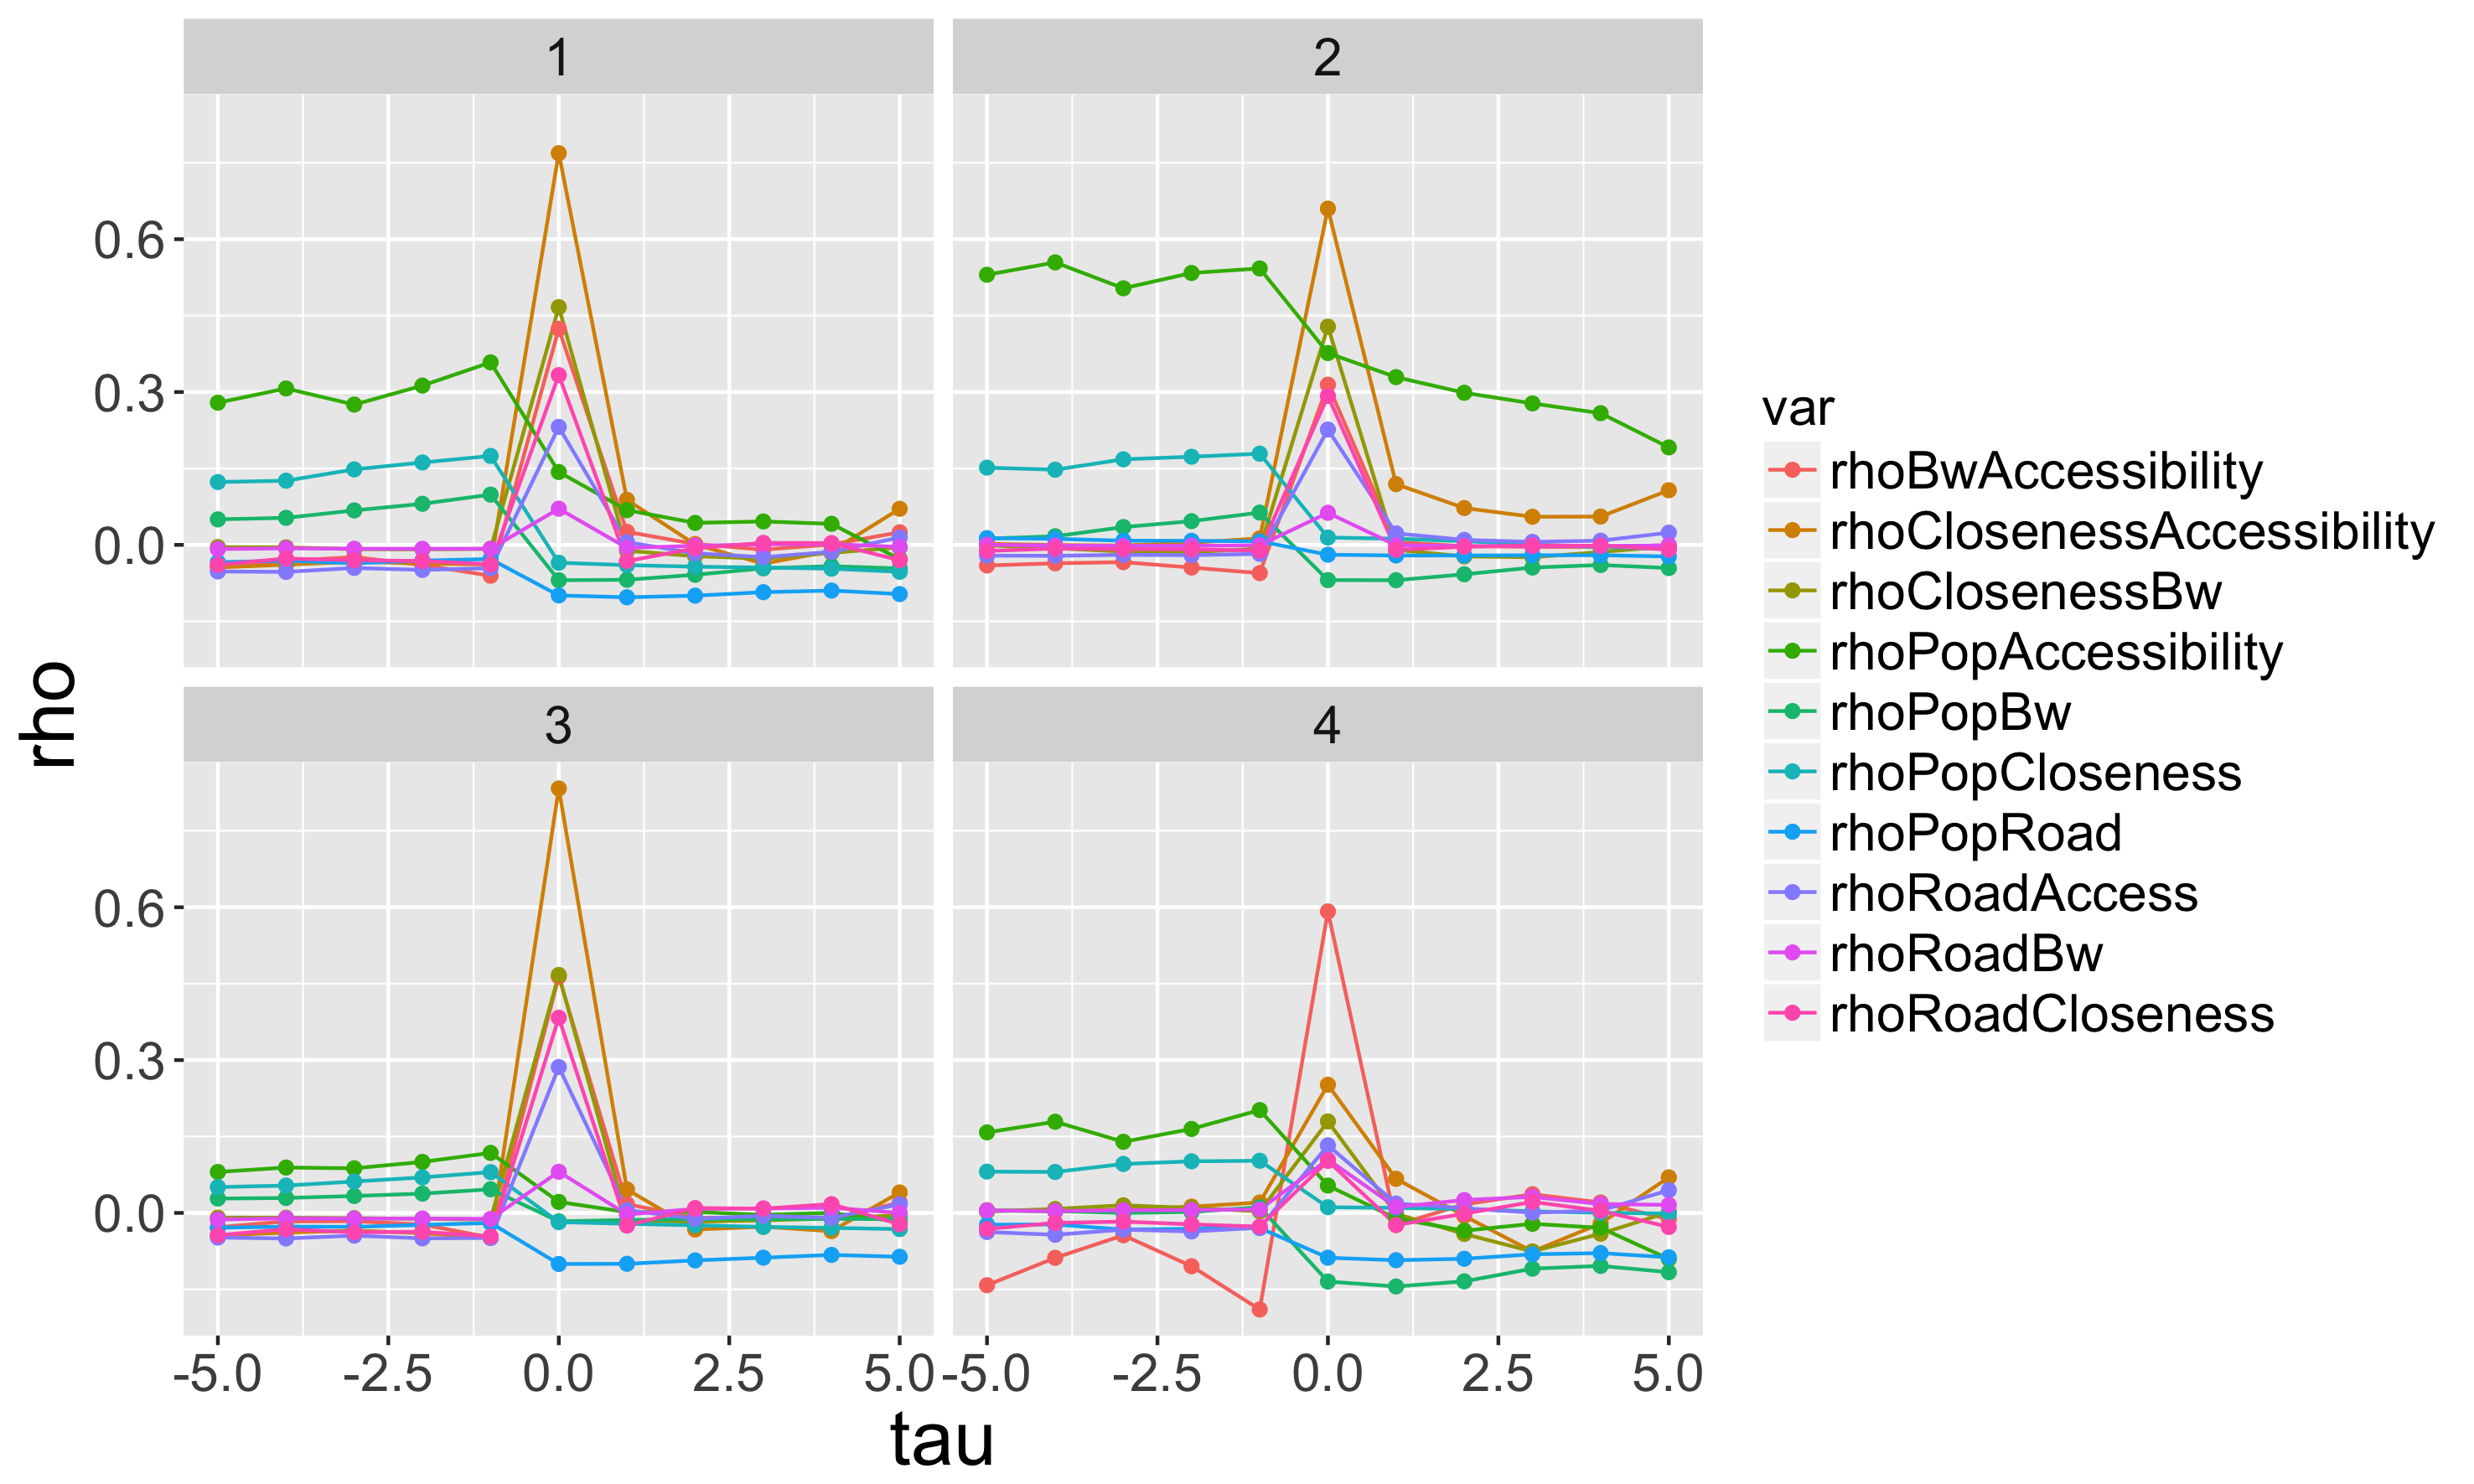
\includegraphics[width=0.53\linewidth]{Figures/MesoCoEvol/centertrajs}
	%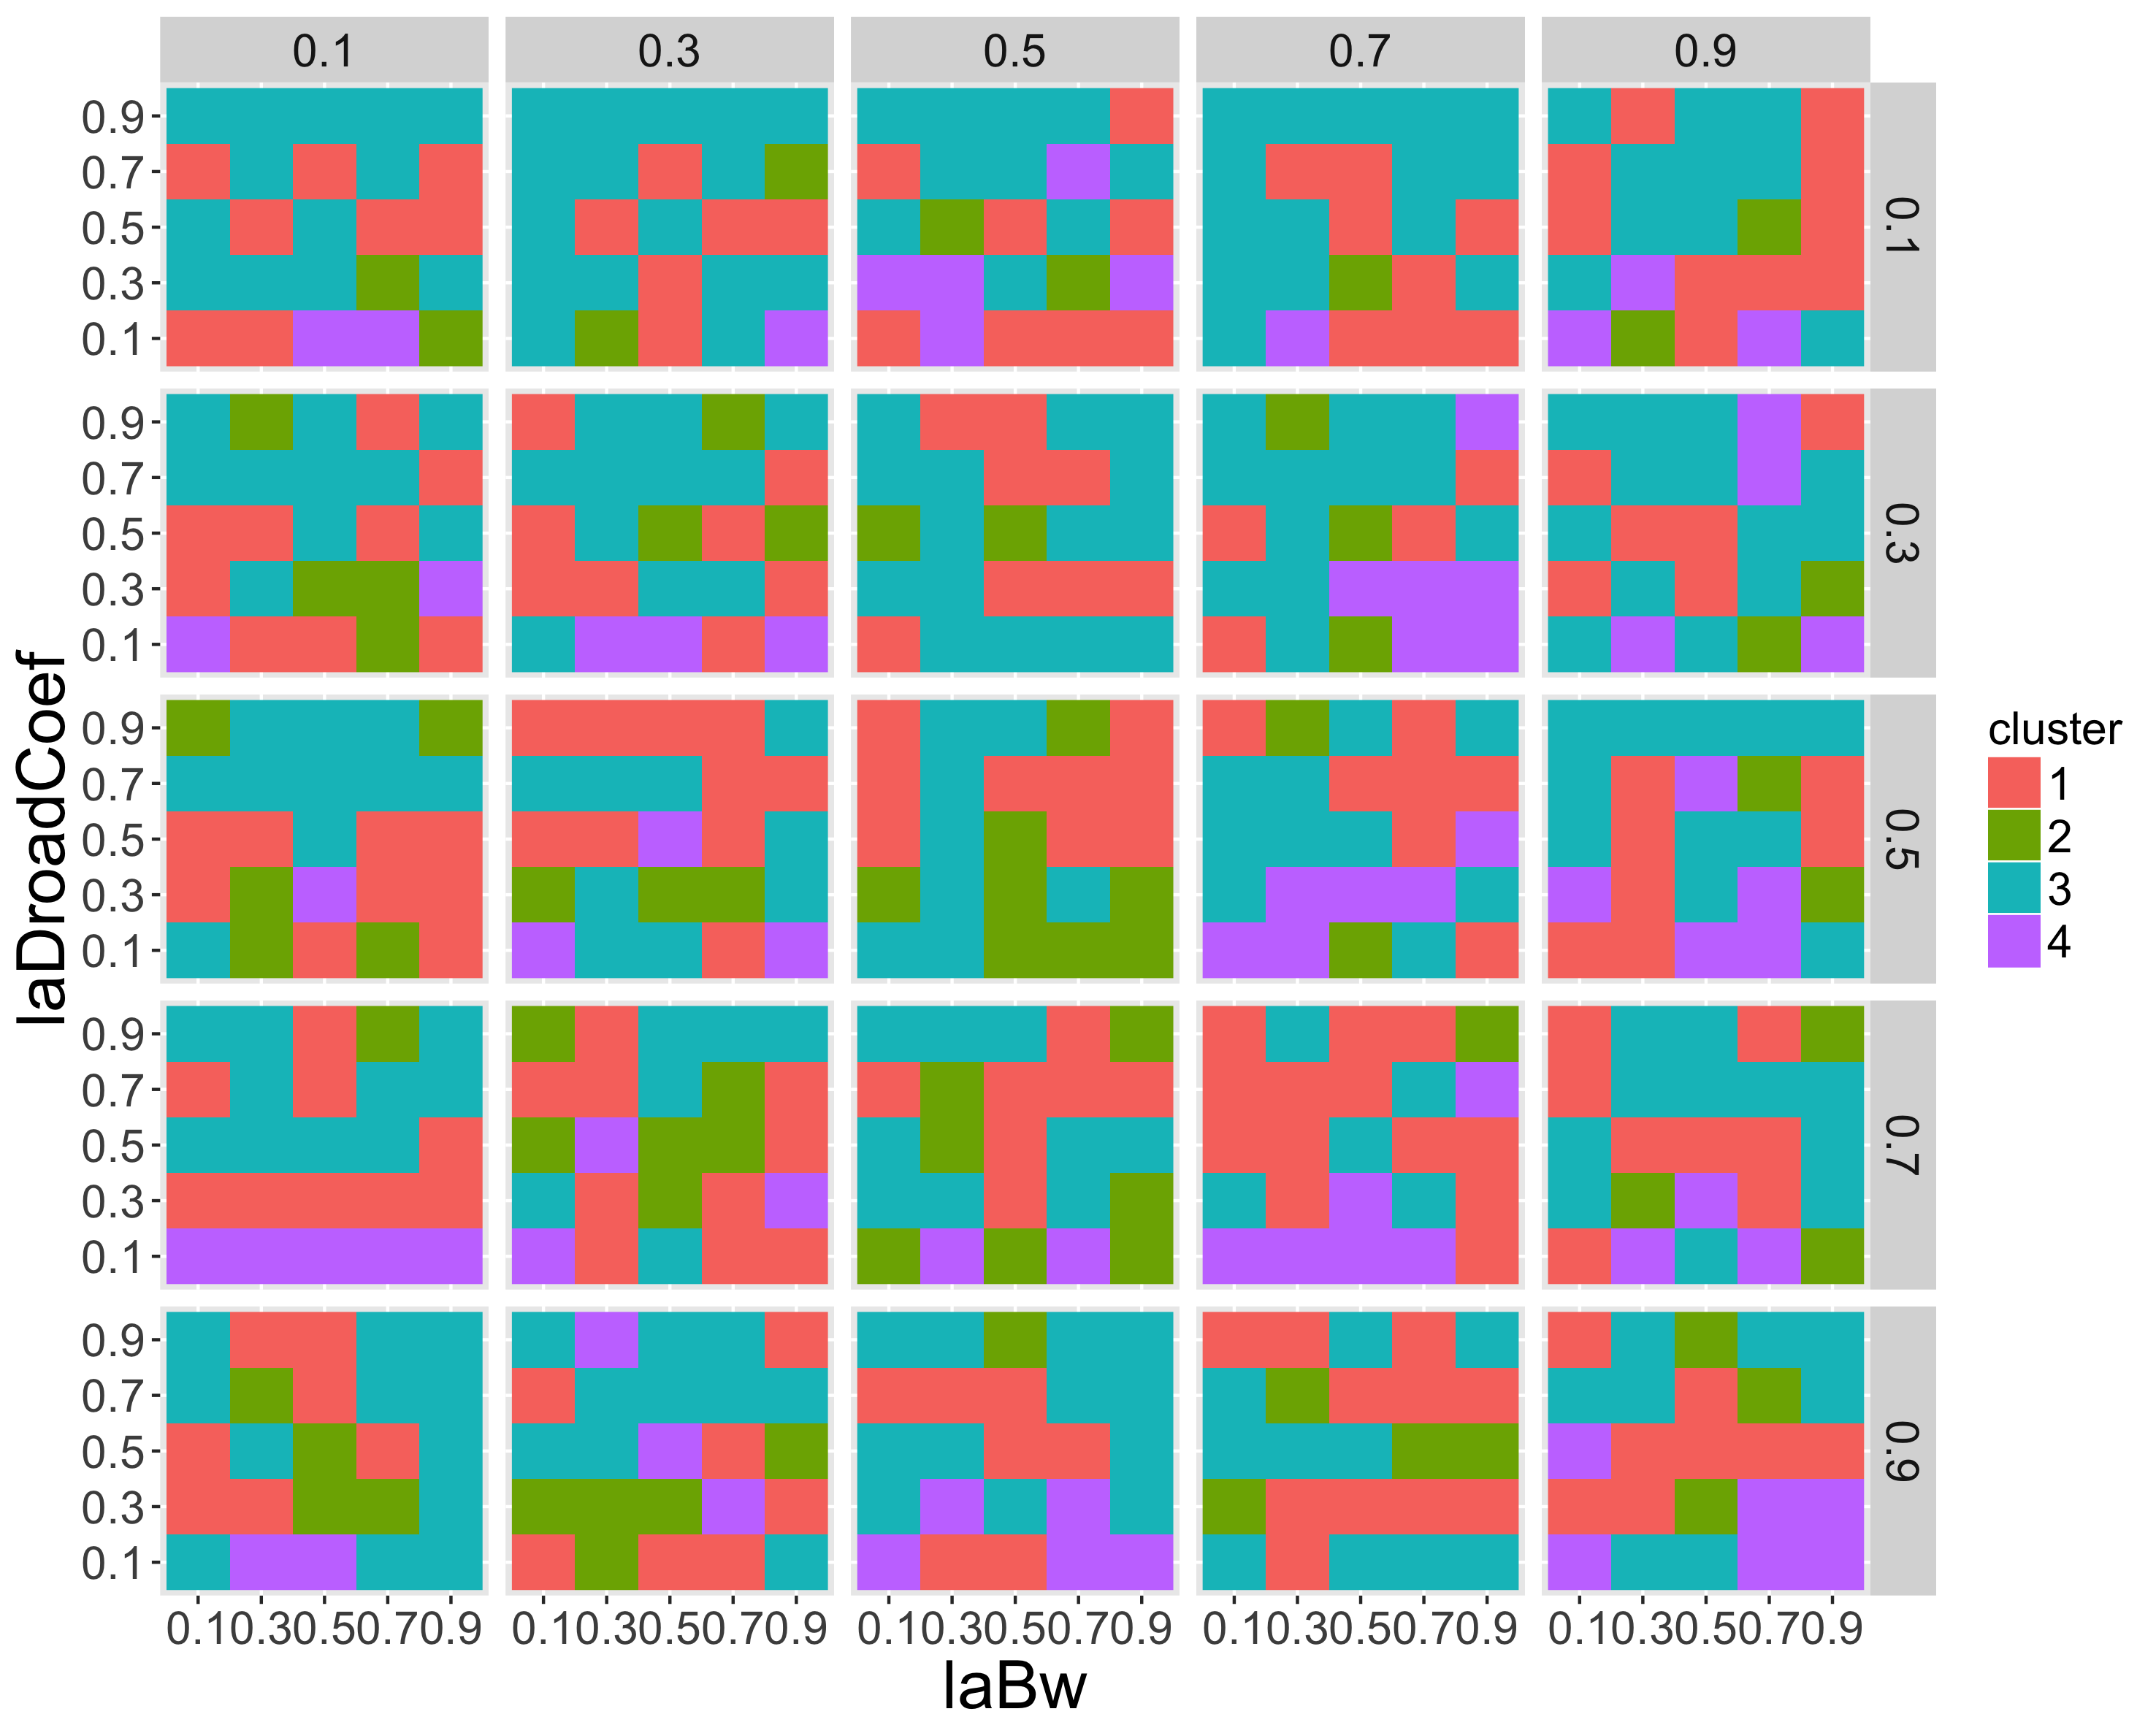
\includegraphics[width=0.44\linewidth]{Figures/MesoCoEvol/cluster-params}
	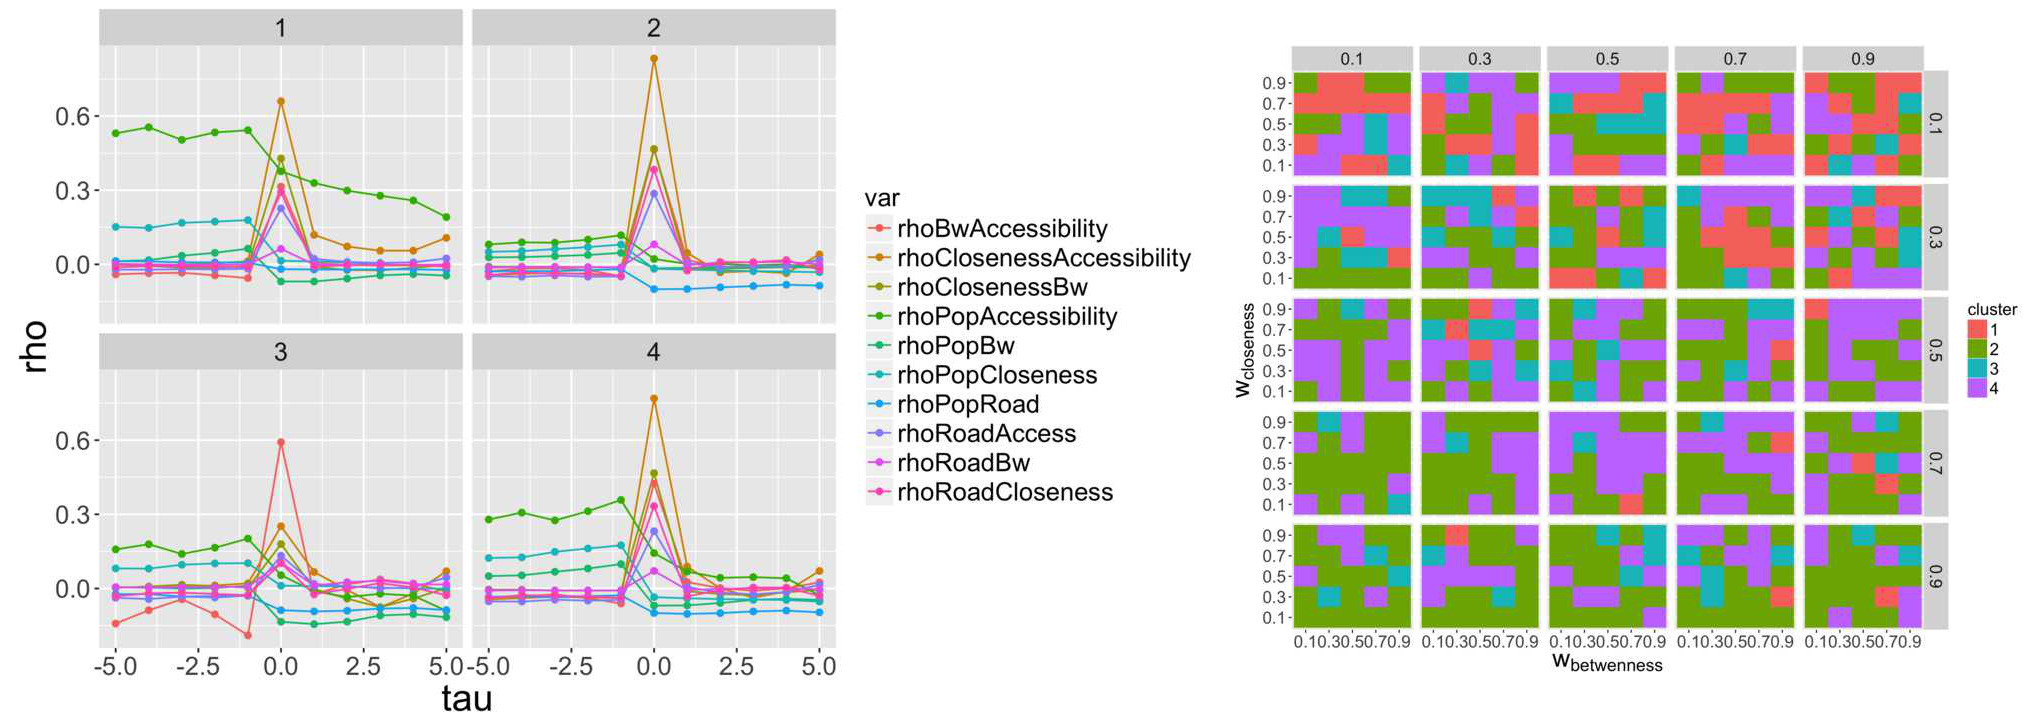
\includegraphics[width=\textwidth]{Figures/Final/7-2-2-fig-mesocoevolmodel-causality}
	\caption[Causality regimes][Régimes de causalité]{}{\textbf{Régimes de causalité.}\label{fig:mesocoevolmodel:causality}}
\end{figure}
%%%%%%%%%%%%%%%





%%%%%%%%%%%%%%%
\subsection{Developments}{Développements}



\comment[JR]{\cite{blumenfeld2010network} : hybrid model (largely discussed by Clara) ; network growth induces migration ; would be interesting to test its abilities to produce various causality regimes (note : may be one indicator of how a model captures co-evolution ?)}


\comment[JR]{develop on Elsa's comment, why just the network with prefatt ? more subtle and want to reproduce coupled dynamics. could suit at the first order ? surely as density-only model performs quite well on morphology only. question of territorial representations, what is necessary, what is an objective, what is both. dimension of urban system.}











